
\documentclass[compress]{beamer}

%\usepackage{beamerthemesplit}
\usepackage{xmpmulti}

\usepackage{graphicx,float,wrapfig, bbm}
\usepackage{amsfonts, bbold, comment}
\usepackage{mdwlist}
\usepackage{subfigure}
\usepackage{colortbl}

\usepackage{multirow}

\pgfdeclareimage[width=\paperwidth]{mybackground}{../../common/boulder.pdf}

\newcommand{\e}[2]{\mathbb{E}_{#1}\left[ #2 \right] }
\newcommand{\ind}[1]{\mathbb{I}\left[ #1 \right] }
\newcommand{\ex}[1]{\mbox{exp}\left\{ #1\right\} }
\newcommand{\g}{\, | \,}

\newcommand{\gfxs}[2]{
\begin{center}
	\includegraphics[width=#2\linewidth]{simtrans/#1}
\end{center}
}

\newcommand{\gfxq}[2]{
\begin{center}
	\includegraphics[width=#2\linewidth]{qb/#1}
\end{center}
}


\usetheme[bullet=circle,                     % Use circles instead of squares for bullets.
          titleline=true,                    % Show a line below the frame title.
          showdate=true,                     % show the date on the title page
          alternativetitlepage=true,         % Use the fancy title page.
          titlepagelogo=general_figures/culogo,              % Logo for the first page.
          % Logo for the header on first page.
          headerlogo=general_figures/boulder_cs,
          ]{UCBoulder}

\usecolortheme{ucdblack}
\title[Thinking on Your Feet]{Thinking on your Feet: Reinforcement Learning for Incremental
Language Tasks}
\author{ Jordan Boyd-Graber}
\date{Fall 2014}

\institute[Boulder] % (optional, but mostly needed)
{University of Colorado Boulder}

\AtBeginSection[] % "Beamer, do the following at the start of every section"
{ \begin{frame} \frametitle{Outline} % make a frame titled "Outline"
\tableofcontents[currentsection] % show TOC and highlight current section
\end{frame} }

\begin{document}

\frame{
\titlepage
\tiny
}


\begin{frame}{Nuremburg Trials}

\begin{columns}

\column{.5\linewidth}

    \gfxs{nuremberg_trials}{1.0}

\column{.5\linewidth}

    \begin{itemize}
        \item Dozens of defendants
        \item Judges from four nations (three languages)
     \end{itemize}

\end{columns}

\end{frame}


\begin{frame}{How Long are you Willing to Wait for a Translation?}

\begin{itemize}
  \item If you have to wait until the person speaking stops talking,
    then they wait for you to finish translating, it can take
    \emph{forever}!
    \pause
   \item Much better \only<3->{if you could get}
     \only<4->{translations as soon as possible}
\end{itemize}

\end{frame}


\begin{frame}{Algorithms that think on their feet}

\begin{columns}

  \column{.65\linewidth}
  \begin{itemize}
     \item Algorithms that process examples \emph{one word at a time}
       \begin{itemize}
         \item Simultaneous machine translation
         \item Trivia games
       \end{itemize}
      \item Similar structure
        \begin{itemize}
          \item Prediction
          \item Policy
        \end{itemize}
  \end{itemize}

  \column{.3\linewidth}

  \gfxs{nuremberg_translators}{.7}
  \gfxq{quizbowl}{.7}

\end{columns}

\end{frame}

\section{Quiz Bowl}

\begin{frame}
	\frametitle{Humans doing Incremental Classification}
	\begin{columns}

	\column{.5\linewidth}
	\begin{itemize}
		\item Game called ``quiz bowl''
		\item Two teams play each other
		\begin{itemize}
			\item Moderator reads a question
			\item When a team knows the answer, they signal (``buzz'' in)
			\item If right, they get points; otherwise, rest of the question is read to the other team
		\end{itemize}
		\item Hundreds of teams in the US alone
                \only<2>{\item Example \dots}
	\end{itemize}

	\column{.5\linewidth}
	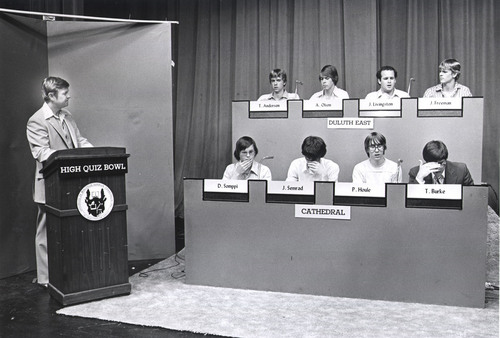
\includegraphics{qb/quizbowl}

	\end{columns}

\end{frame}

\begin{comment}

\begin{frame}[t]
	\frametitle{Sample Question 1}

With Leo Szilard, he invented a doubly-eponymous \only<2->{refrigerator with no moving parts. He did not take interaction with neighbors into account when formulating his theory of} \only<3->{heat capacity, so} \only<4->{Debye adjusted the theory for low temperatures. His} \only<4->{summation convention automatically sums repeated indices in tensor products. His name is attached to the A and B coefficients} \only<5->{for spontaneous and stimulated emission, the subject of one of his multiple groundbreaking 1905 papers. He further developed the model of statistics sent to him by} \only<6->{Bose to describe particles with integer spin. For 10 points, who is this German physicist best known for formulating the} \only<7->{special and general theories of relativity?} \\
\vspace{1cm}
\only<8->{ {\bf Albert \underline{Einstein}}}
\end{frame}

\end{comment}


\begin{frame}[t]
\frametitle{Sample Question}

One is Monte Carlo if at least half of the possible results for all x in a
\only<2->{language it says ``yes'' and ``no'' otherwise. One is called} \only<3->{unambiguous if for any $x$ there is at most one accepting computation. One is
called} \only<4->{oblivious if the position of the} \only<5->{cursor at the $t^{th}$
step depends only on the $t$ and the length of the input. One is} \only<6->{non-deterministic if its sets of next} \only<7->{states may contain more than one
element. For ten points, identify this model of} \only<8->{computation named for
an} \only<9->{English computer scientist.} \\
\only<10->{{\bf ANSWER: \underline{Turing} Machine (prompt on TM)}}


\end{frame}


\begin{frame}
	\frametitle{Humans doing Incremental Classification}

	\begin{columns}
		\column{.5\linewidth}

		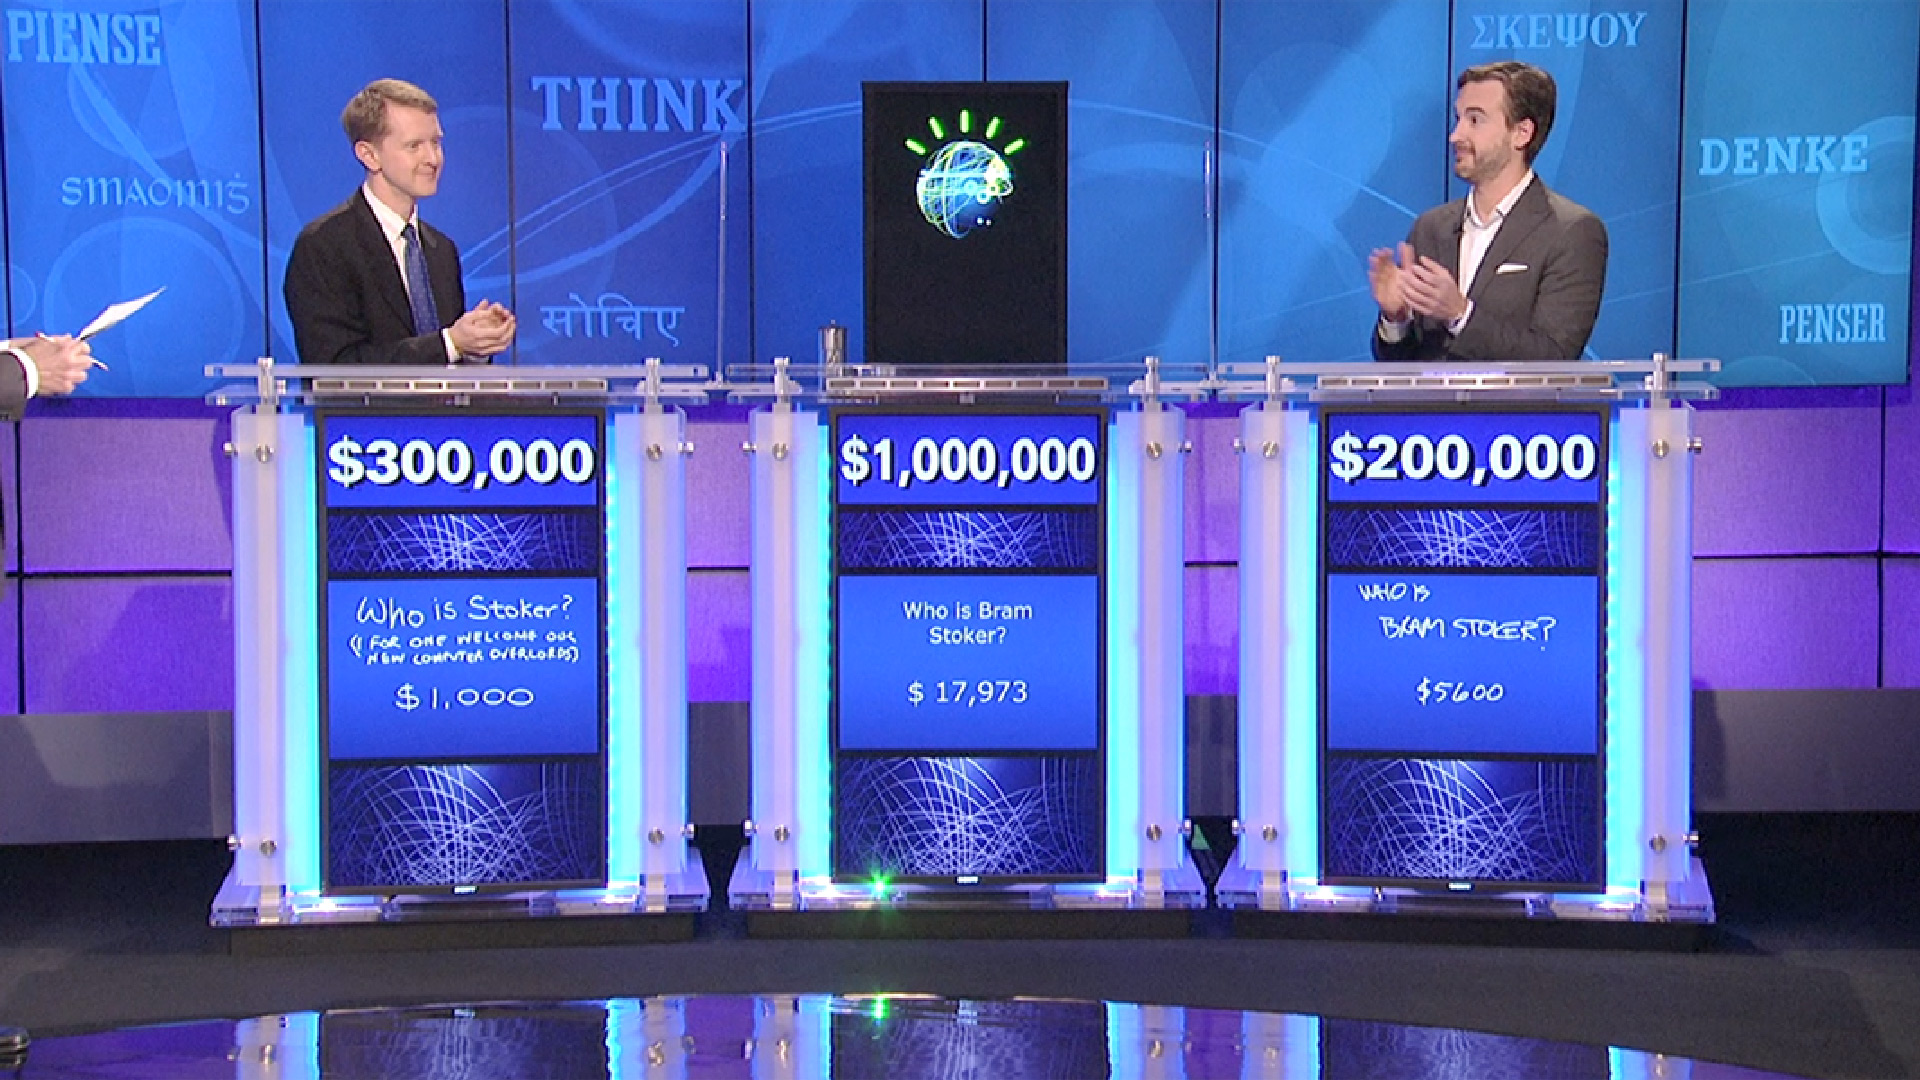
\includegraphics[width=1.0\linewidth]{qb/jeopardy}


		\column{.5\linewidth}
		\begin{itemize}
			\item This is {\bf not} Jeopardy \cite{ferruci-10}
			\item There are buzzers, but players can only buzz at the end of a question
			\item Doesn't discriminate knowledge
			\item Quiz bowl questions are pyramidal
		\end{itemize}

	\end{columns}

\end{frame}



\begin{frame}
	\frametitle{Humans doing Incremental Classification}

	\begin{itemize}
		\item Thousands of questions are written every year
		\item Large question databases
		\item Teams practice on these questions (some online, e.g. IRC)
		\item How can we use this process?
	\end{itemize}

\end{frame}


\begin{frame}

\frametitle{Interface}

\begin{columns}

	\column{0.5\linewidth}

	\begin{center}
		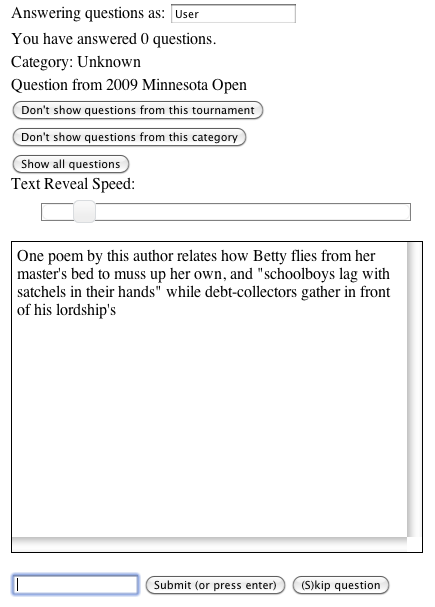
\includegraphics[width=0.8\linewidth]{qb/screenshot}
	\end{center}

	\column{0.5\linewidth}
	\only<1>{
	\begin{itemize}
		\item Users could ``veto'' categories or tournaments
		\item Questions presented in canonical order
		\item Approximate string matching (w/ override)
	\end{itemize}
	}

	\only<2>{
	\begin{itemize}
		\item Started on Amazon Mechanical Turk
		\item 7000 questions were answered in the first day
		\item Over 43000 questions were answered in the space of two weeks
		\item Total of 461 unique users
		\item Leaderboard to encourage users
	\end{itemize}
	}

\end{columns}
\end{frame}


\begin{frame}
	\frametitle{Accuracy vs. Speed}

	\begin{center}
	  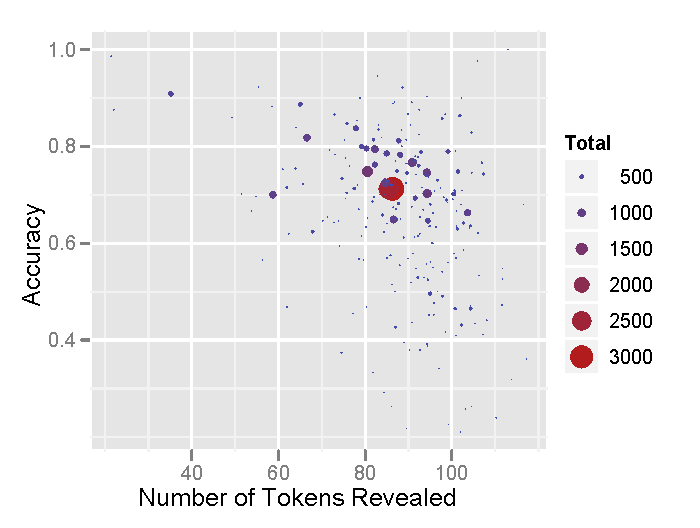
\includegraphics[width=0.8\linewidth]{qb/accuracy_vs_speed}
	  \end{center}

\end{frame}


\begin{frame}
	\begin{center}

\vspace{-.6cm}
\begin{figure}[tb]
\centering

\subfigure[Buzzes over all Questions]{
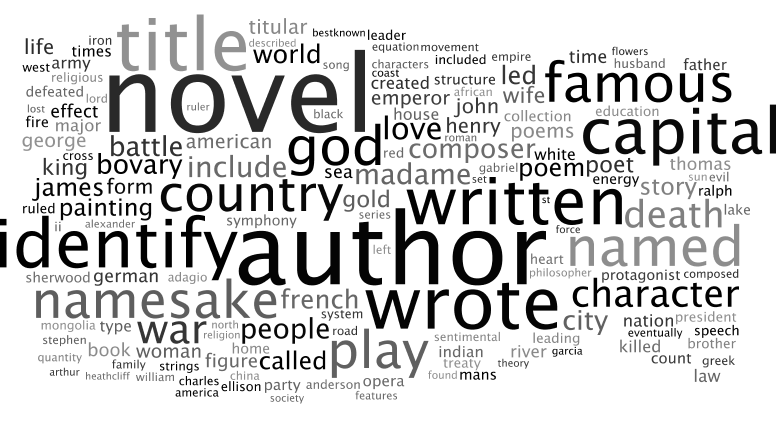
\includegraphics[width=0.6\linewidth]{qb/buzz_cloud}
\label{fig:buzz_cloud}
}

\subfigure[Wuthering Heights Question Text]{
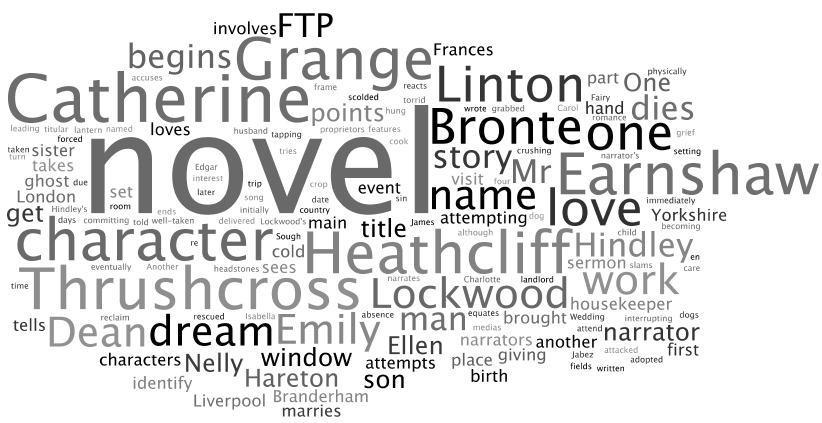
\includegraphics[width=0.45\linewidth]{qb/wuthering_heights_question}
\label{fig:wh_question}
}
\subfigure[Buzzes on Wuthering Heights]{
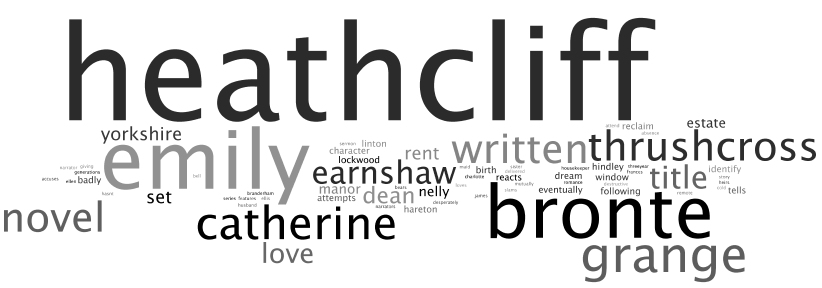
\includegraphics[width=0.45\linewidth]{qb/wuthering_heights_buzz}
\label{fig:wh_buzz}
}
\end{figure}


	\end{center}

\end{frame}


\begin{frame}
	\frametitle{System for Incremental Classifiers}

	\begin{itemize}
		\item Treat this as a MDP
		\item Action: {\bf buzz} now or {\bf wait}
                     \pause
                    \begin{enumerate}
                  \item {\bf Content Model} is constantly generating guesses
                     \item {\bf Oracle} provides examples where it is correct
                   \item The {\bf Policy} generalizes to test data
                       \item {\bf Features} represent our state
                    \end{enumerate}
	\end{itemize}
\begin{block}{}
  \begin{center}
    \vspace{-.5cm}
    \begin{tabular}{cccc}
      \alert<3->{content model} & oracle & policy & features \\
    \end{tabular}
    \vspace{-.5cm}
  \end{center}
\end{block}
\end{frame}


\begin{frame}{Content Model}

\begin{block}{}
  \begin{center}
    \vspace{-.5cm}
    \begin{tabular}{cccc}
      \alert{content model} & oracle & policy & features \\
    \end{tabular}
    \vspace{-.5cm}
  \end{center}
\end{block}


  \begin{itemize}
   \item Bayesian generative model with answers as latent state
         \item Unambiguous Wikipedia pages
           \item Unigram term weightings (na\"ive Bayes, BM25)
    \item Maintains posterior distribution over guesses
    \item Always has a guess of what it should answer
      \begin{itemize}
        \item policy will tell us when to trust it
       \end{itemize}

  \end{itemize}
\end{frame}

\begin{frame}{Vector Space Model}

  \only<1>{\gfxq{unigram_models_0}{.8}}
  \only<2>{\gfxq{unigram_models_1}{.8}}
  \only<3>{\gfxq{unigram_models_2}{.8}}
  \only<4>{\gfxq{unigram_models_3}{.8}}
  \only<5>{\gfxq{unigram_models_4}{.8}}
  \only<6>{\gfxq{unigram_models_5}{.8}}
  \only<7>{\gfxq{unigram_models_6}{.8}}
  \only<8>{\gfxq{unigram_models_7}{.8}}
  \only<9>{\gfxq{unigram_models_8}{.8}}


\end{frame}

\begin{frame}{Oracle}
\begin{block}{}
  \begin{center}
    \vspace{-.5cm}
    \begin{tabular}{cccc}
      content model & \alert{oracle} & policy & features \\
    \end{tabular}
    \vspace{-.5cm}
  \end{center}
\end{block}
\begin{center}
  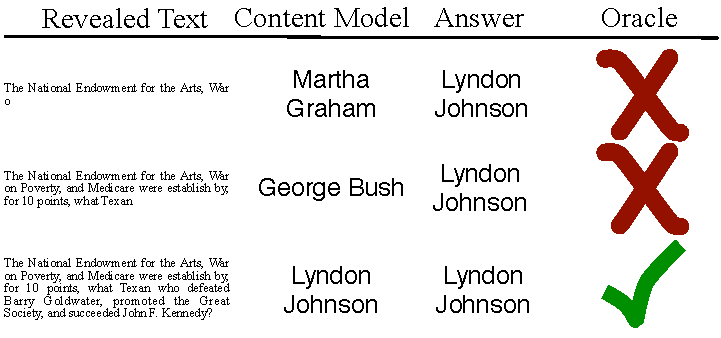
\includegraphics[width=0.8\linewidth]{qb/oracle}
\end{center}

\begin{itemize}
  \item As each token is revealed, look at content model's guess
    \item If it's right, positive instance; otherwise negative
      \item Nearly optimal policy to buzz whenever correct (upper bound)
\end{itemize}

\end{frame}

\begin{frame}{Policy}

\begin{block}{}
  \begin{center}
    \vspace{-.5cm}
    \begin{tabular}{cccc}
      content model & oracle & \alert{policy} & features \\
    \end{tabular}
    \vspace{-.5cm}
  \end{center}
\end{block}

 \begin{itemize}
    \item Mapping: state $\mapsto$ action
    \item Use oracle as example actions
    \item Learned as classifier \cite{langford-05}
    \item At test time, use the same features as for training
      \begin{itemize}
        \item Question text (so far)
        \item Guess
        \item Posterior distribution
        \item Change in posterior
      \end{itemize}
\end{itemize}

\end{frame}



\begin{frame}[t]{Features (by example)}

\only<1-3>{
\begin{block}{}
  \begin{center}
    \vspace{-.5cm}
    \begin{tabular}{cccc}
      content model & oracle & policy & \alert{features} \\
    \end{tabular}
    \vspace{-.5cm}
  \end{center}
\end{block}
\vspace{.5cm}
}

\only<4->{\vspace{-1.5cm}}

  \begin{columns}[T]
    \column{.3\linewidth}

    \only<1->{ 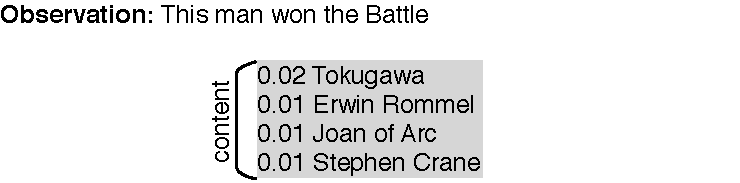
\includegraphics[width=2\linewidth]{qb/feature_ex_l_1} \\ }
    \vspace{.5cm}
    \only<4->{ 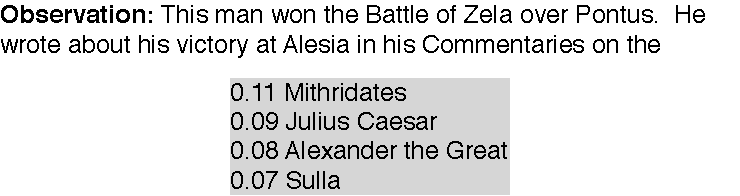
\includegraphics[width=2\linewidth]{qb/feature_ex_l_2}  \\ }
    \vspace{.5cm}
    \only<7->{ 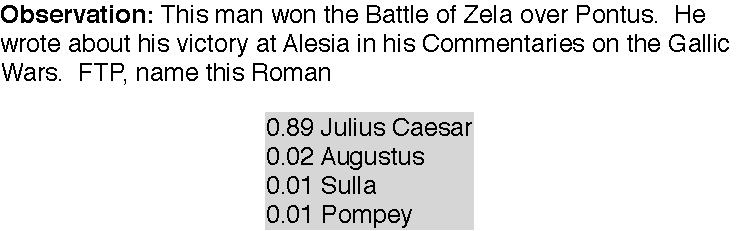
\includegraphics[width=2\linewidth]{qb/feature_ex_l_3}  \\ }


    \column{.68\linewidth}
    \vspace{-.5cm}
    \only<2->{ 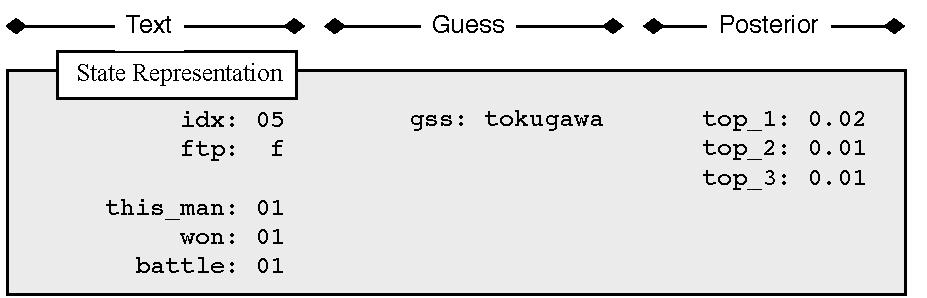
\includegraphics[width=.85\linewidth]{qb/feature_ex_r_1} \\ }
    \only<3->{ \vspace{-.5cm} \hspace{.5cm} 
\includegraphics[width=.1\linewidth]{qb/feature_ex_wait}  \\ }
    \only<5->{ 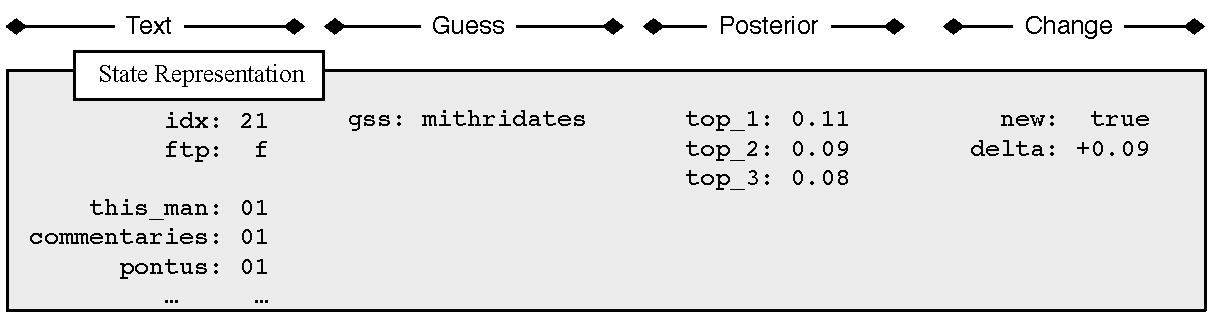
\includegraphics[width=\linewidth]{qb/feature_ex_r_2} \\ }
    \only<6->{ \vspace{-.5cm} \hspace{.5cm}
\includegraphics[width=.1\linewidth]{qb/feature_ex_wait}  \\ }
    \only<8->{ 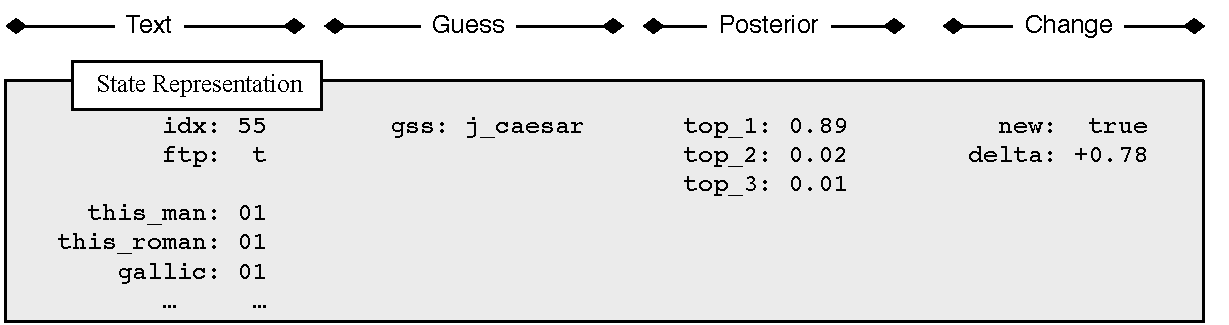
\includegraphics[width=\linewidth]{qb/feature_ex_r_3} \\ }
    \only<9->{ \vspace{-.5cm} \hspace{.5cm} 
\includegraphics[width=.1\linewidth]{qb/feature_ex_buzz}  \\ }
    \only<9->{Answer: {\bf Julius Caesar}}
  \end{columns}

\end{frame}



\begin{frame}{Simulating a Game}
		\begin{itemize}
			\item Present tokens incrementally to algorithm, see where it buzzes
			\item Compare to where humans buzzed in
			\item Payoff matrix (wrt Computer)
			\begin{center}
\begin{tabular}{lccr}
& Computer & Human & Payoff \\
\hline
1 & first and wrong & right & $-15$ \\
2 & --- & first and correct & $-10$ \\
3  & first and wrong & wrong & $-5$ \\
4 & first and correct & --- & $+10$ \\
5 & wrong & first and wrong & $+5$ \\
6 & right & first and wrong & $+15$ \\
\hline
\end{tabular}
			\end{center}
		\end{itemize}
\end{frame}



\begin{frame}{Simulating a Game}

  \begin{itemize}
    \item What human actions to compare against?
      \invisible<1>{
      \begin{itemize}
        \item On each question, take the {\bf median} buzz (more in paper)
      \end{itemize}
      }
     \item Does it to better than obvious rapacious baselines?
      \invisible<-2>{
        \begin{itemize}
          \item Yes---experiments in paper
          \end{itemize}
        }
    \item How do features affect performance?
      \invisible<-3>{
      \begin{itemize}
        \item Nothing hurts, but only a handful help (details in paper)
      \end{itemize}
      }
  \end{itemize}

  \invisible<-4>{.}

\end{frame}


\begin{frame}[t]

\frametitle{Error Analysis}

\begin{columns}

	\column{.4 \linewidth}
        \only<5-> {

		\begin{itemize}
			\item \alert<5> { Too slow }
			\item \alert<6> {Coreference \cite{haghighi-07} and correct question
type \cite{moldovan-00}}
			\item \alert<7> {Not enough information / not weighting later clues higher }
		\end{itemize}

}

	\column{.6 \linewidth}

		\begin{center}
			\only<1>{  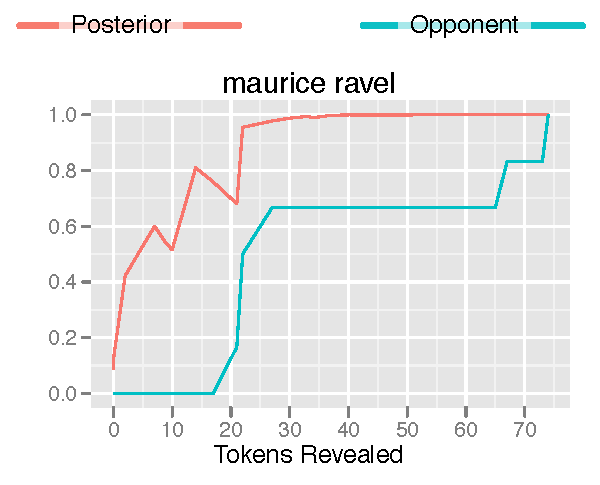
\includegraphics[width=.9\linewidth]{qb/real_question_ravel_0} \\ }
			\only<2>{  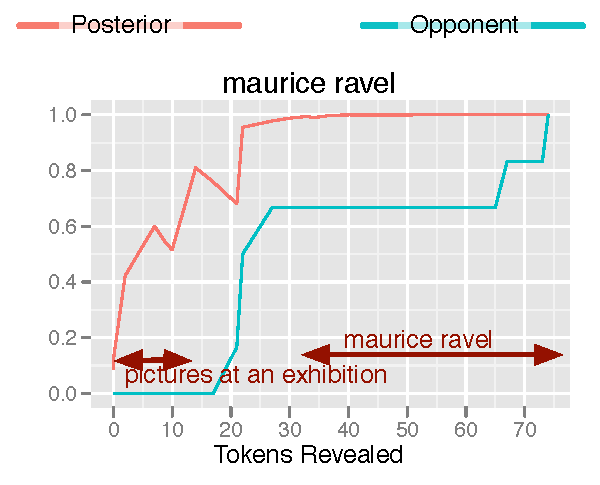
\includegraphics[width=.9\linewidth]{qb/real_question_ravel_1} \\ }
			\only<3>{  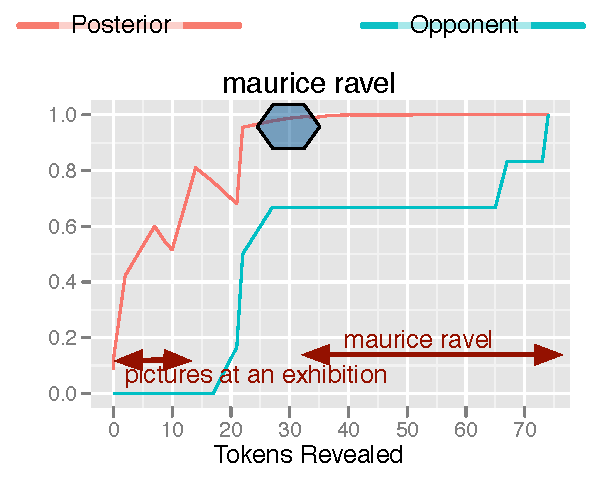
\includegraphics[width=.9\linewidth]{qb/real_question_ravel_2}
                          \\ }
			\only<4-5>{  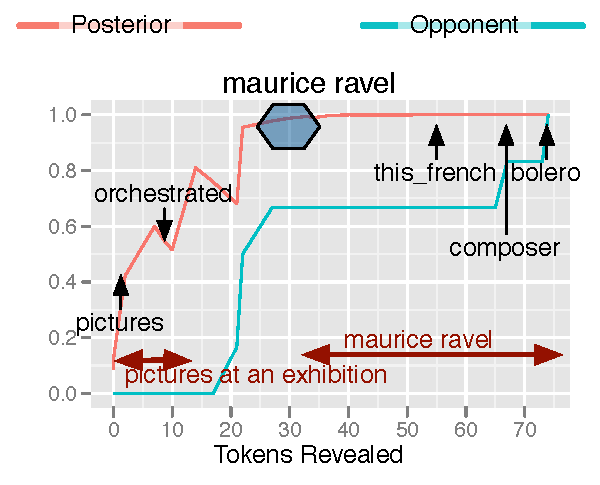
\includegraphics[width=.9\linewidth]{qb/real_question_ravel_3} \\ }
			\only<6>{  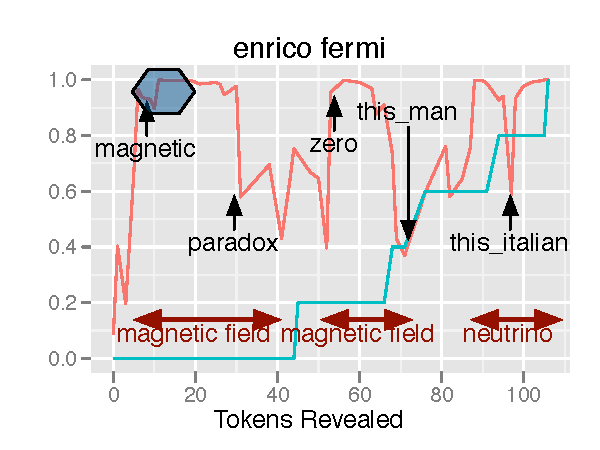
\includegraphics[width=.9\linewidth]{qb/real_question_fermi} \\ }
			\only<7>{  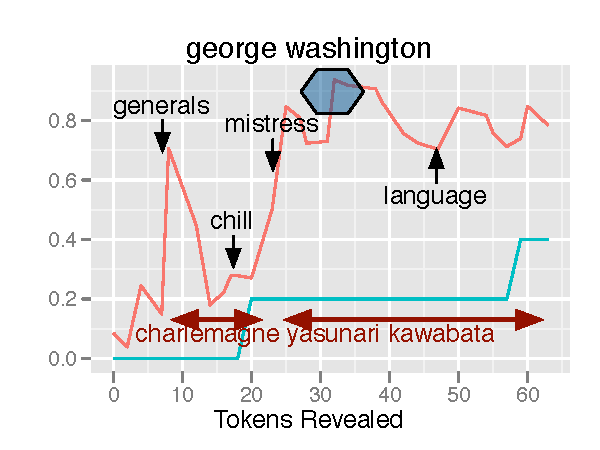
\includegraphics[width=.9\linewidth]{qb/real_question_washington} \\ }
			\only<2>{ 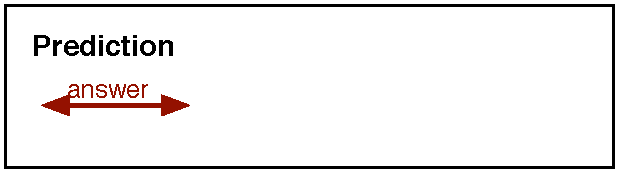
\includegraphics[width=.9\linewidth]{qb/real_question_key_0} }
			\only<3>{ 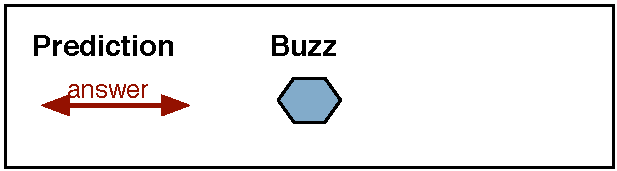
\includegraphics[width=.9\linewidth]{qb/real_question_key_1} }
			\only<4->{ 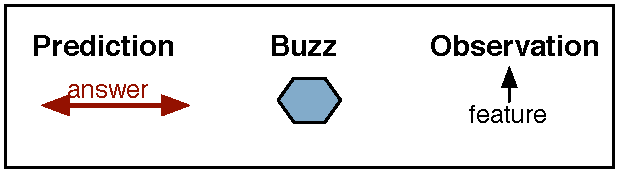
\includegraphics[width=.9\linewidth]{qb/real_question_key_2} }
		\end{center}
\end{columns}

\end{frame}

\begin{frame}{How can we do better?}

  \begin{itemize}
    \item Use order of words in a sentence ``this man shot at Aaron
      Burr'' very different from ``Aaron Burr shot at this man''
    \item Use relationship between questions (``China'' and
      ``Taiwan'')
    \item Use learned features
      \pause
    \item Recursive Neural Networks (Socher et al, 2010)
  \end{itemize}

\end{frame}

\begin{frame}{Using Compositionality}

  \only<1-2>{\gfxq{rnn_11}{.8}}
  \only<3>{\gfxq{rnn_10}{.8}}
  \only<4>{\gfxq{rnn_9}{.8}}
  \only<5>{\gfxq{rnn_8}{.8}}
  \only<6>{\gfxq{rnn_7}{.8}}
  \only<7>{\gfxq{rnn_6}{.8}}
  \only<8>{\gfxq{rnn_5}{.8}}
  \only<9>{\gfxq{rnn_4}{.8}}
  \only<10>{\gfxq{rnn_3}{.8}}
  \only<11>{\gfxq{rnn_2}{.8}}
  \only<12>{\gfxq{rnn_1}{.8}}
  \only<13>{\gfxq{rnn_0}{.8}}
\end{frame}

\section{Simultaneous Translation}

\begin{frame}{Simultaneous translation is the norm}

  \begin{columns}
    \column{.5\linewidth}
       \gfxs{nuremberg_translators}{.9}
    \column{.5\linewidth}
       \begin{itemize}
         \item Rigorous training
         \item Technological sophistication
         \item Long way from ``sentence at a time''
       \end{itemize}
  \end{columns}

\end{frame}

\begin{frame}{Why simultaneous translation really hard is}

  \begin{columns}
    \column{.5\linewidth}
      \begin{itemize}
        \item Many languages are \textsc{sov}
        \item \alert<2>{German}, Japanese, Farsi, Korean, \alert<3>{Yiddish}
      \end{itemize}
    \column{.5\linewidth}
      \gfxs{yoda}{.6}
  \end{columns}

  \centering

\only<4->{
\vspace{1cm}

\begin{tabular}{c@{ }c@{ }c@{ }c@{ }c@{ }c@{ }c@{ }l}
ich & bin & mit & dem & Zug & nach & Ulm & {\bf gefahren} \\
I & am & with & the & train & to & Ulm & {\bf traveled} \\
\hline
I & \multicolumn{6}{c}{\emph{(\dots\dots waiting\dots\dots)}} & {\bf traveled} by train to Ulm \\
\end{tabular}
}

\end{frame}

\begin{frame}{Solution: Predicting the Verb}

\begin{columns}

\column{.5\linewidth}
  \begin{itemize}
    \item If we can figure out the verb, we can ``complete'' the
      sentence
    \item This is provided by language models that can predict the
      next word in a sentence
    \item Instead, we'll predict the verb
  \end{itemize}

\column{.5\linewidth}

\gfxs{autocomplete}{.8}

\end{columns}

\end{frame}


\begin{frame}{Language Models of Verbs}

  \only<1>{\gfxs{verb_corpus_1}{.9}}
  \only<2>{\gfxs{verb_corpus_2}{.9}}
  \only<3>{\gfxs{verb_corpus_3}{.9}}

\end{frame}

\begin{frame}{Predicting the Verb}
\begin{itemize}
  \item Build language model for every verb
  \item Then, for any input text $x$ we can make a prediction of the verb
\begin{equation}
  \arg\max_v p(v) \prod_{i=1}^t p(x_i \g v, x_{i-n+1:i-1})
\end{equation}
\pause
  \item Most of these predictions will be totally wrong \dots
  \item leading to horrible translations
\end{itemize}
\end{frame}

\begin{frame}{What can we do?}

\begin{columns}

  \column{.5\linewidth}
  \begin{itemize}
    \item We have a set of \alert<2>{actions} (predict / translate)
    \item In a changing environment \only<2->{\alert<2>{(state)}}
    \item With a well defined \alert<2>{reward}
\only<3>{\item Reinforcement learning}
  \end{itemize}
  \column{.5\linewidth}
  \only<3->{
  \gfxs{pancake_robot}{.8}
  \begin{center}
  Reinforcement Learning in Robotics: Applications and Real-World
  Challenges
  \end{center}
  }

  \end{columns}
\end{frame}

\begin{frame}{States and Actions}

  \begin{itemize}
    \item State
      \begin{itemize}
        \item The words we've seen
        \item Predictions
      \end{itemize}
      \pause
    \item Actions
      \begin{itemize}
        \item Wait
        \item \alert<3>{Predict Verb}
        \item \alert<3>{Predict Next Word}
        \item \alert<3>{Commit}
      \end{itemize}
    \end{itemize}
\end{frame}

\begin{frame}{Translations}
  \begin{itemize}
    \item Assume a ``black box''
    \item German in, English out
  \end{itemize}

\end{frame}

\begin{frame}{Consensus Translation}

  \only<1>{\begin{center}
``German in, English out'' black box
      \end{center}}

  \only<2>{\gfxs{consensus_0}{.8}}
  \only<3>{\gfxs{consensus_1}{.8}}
  \only<4>{\gfxs{consensus_2}{.8}}
  \only<5>{\gfxs{consensus_3}{.8}}
  \only<6>{\gfxs{consensus_4}{.8}}

\end{frame}

\begin{frame}{How we could translate a sentence}

\only<1>{\gfxs{example_3}{.9}}
\only<2>{\gfxs{example_4}{.9}}
\only<3>{\gfxs{example_5}{.9}}
\only<4>{\gfxs{example_6}{.9}}
\only<5>{\gfxs{example_7}{.9}}
\only<6>{\gfxs{example_8}{.9}}
\only<7>{\gfxs{example_9}{.9}}
\only<8>{\gfxs{example_10}{.9}}
\only<9>{\gfxs{example_11}{.9}}
\only<10>{\gfxs{example_12}{.9}}
\only<11>{\gfxs{example_13}{.9}}
\only<12>{\gfxs{example_14}{.9}}
\only<13>{\gfxs{example_15}{.9}}
\only<14>{\gfxs{example_16}{.9}}
\only<15>{\gfxs{example_17}{.9}}
\only<16>{\gfxs{example_18}{.9}}
\only<17>{\gfxs{example_19}{.9}}
\end{frame}

\begin{frame}{Scoring Translations}
  \only<1>{\gfxs{bleu_ex}{.8}}
  \only<2>{\gfxs{bleu_correlation}{.6}}
  \only<3>{\gfxs{integral_0}{.95}}
  \only<4>{\gfxs{integral_1}{.95}}
\end{frame}

\begin{frame}{Comparing Policies}

  \only<1>{\gfxs{reward_example_0}{.8}}
  \only<2>{\gfxs{reward_example_1}{.8}}
  \only<3>{\gfxs{reward_example_2}{.8}}
  \only<4>{\gfxs{reward_example_3}{.8}}
  \only<5>{\gfxs{reward_example_4}{.8}}
  \only<6>{\gfxs{reward_example_5}{.8}}
  \only<7>{\gfxs{reward_example_6}{.8}}
\end{frame}

\begin{frame}{Imitation Learning}

  \begin{columns}
    \column{.5\linewidth}
       \gfxs{imitation_fold}{.8}
       \gfxs{imitation_drive}{.8}
    \column{.5\linewidth}
    \begin{itemize}
      \item Given all the predictions that we make (and the resulting
        translations) \dots
      \item Discover the optimal in hindsight policies
      \item Goal: Teach our algorithm to think on its feet
      \item Challenge: Represent states in a way that will generalize
    \end{itemize}

  \end{columns}

\end{frame}

\begin{frame}{How do we find a good policy?}

  \begin{itemize}
    \item Find optimal policies through dynamic programming $\pi_0
      \equiv \pi*$
    \item Represent states $s$ through a feature vector $\vec f(s)$
      \pause
    \item Until convergence:
      \begin{itemize}
        \item Generate examples of state action pairs: $(\pi_t(s), s)$
        \item Create a classifier that maps states to actions (an
          apprentice policy) $h_t: f(s) \mapsto A$ \only<3->{(Loss of
            classifier is the negative reward)}
    \item Interpolate learned classifier $\pi_{t+1} = \lambda \pi_t +
      (1-\lambda) h_t$
  \end{itemize}
  \end{itemize}

\only<4->{
  \begin{center}
    \textsc{searn}: \underline{Se}arching to L\underline{earn}
    (Daum\'e \& Marcu, 2006)
    \end{center}
}
\end{frame}


\begin{frame}{Learned Policy}

  \gfxs{learned_policy}{.8}

\end{frame}

\begin{frame}{Example Sentence}

  \gfxs{ex_imperfect}{.7}

\end{frame}

\begin{frame}{Future Steps}

  \begin{itemize}
    \item Richer translation model
    \item Paraphrase database
    \item Verb prediction through argument structure
  \end{itemize}

\end{frame}








	

\begin{frame}
	\frametitle{Learning which Features are Useful}

	\begin{itemize}
		\item Use how humans these data as a prior for supervised maxent model~\cite{daume-04}
		\item Prior for label $a$ and feature $f$ is a function of the number of buzzes $b$ and tf-idf~\cite{salton-68}
\begin{equation}
  \left[ \vphantom{\frac{a}{b}}\alpha \alert<4>{\ind{ b(a,f) > 0}} + \beta \alert<3>{ b(a,f)} + \gamma
  \right] \alert<2>{\mbox{tf-idf}(a,f)} .
\label{eq:meanweight}
\end{equation}
		\begin{itemize}
			\item $\alpha$, $\beta$, and $\gamma = 0$: na\"ive zero prior
			\item $\alpha$ and $\beta = 0$: linear transformation of the mean
			\item $\alpha$ and $\gamma = 0$: number of buzzes times tf-idf value of the features
		\end{itemize}

	\end{itemize}

\end{frame}

\begin{frame}
	\frametitle{Using buzzes as a prior}

\begin{equation*}
  \left[ \vphantom{\frac{a}{b}}\alpha \ind{ b(a,f) > 0} + \beta b(a,f) + \gamma
  \right] \mbox{tf-idf}(a,f) .
\end{equation*}

\begin{center}
\begin{tabular}{cccccc}
Answers & Weighting & $\alpha$ & $\beta$ & $\gamma$ & Error\footnote{Buzz and tf-idf computed on training data; grid search on dev data; error on test data} \\
\hline
\multirow{5}{*}{100} & zero & - & - & - & 0.22 \\
& tf-idf & - & - & 8.3 & 0.08 \\
&  buzz-binary & 10.7 & - & - & {\bf 0.06} \\
&  buzz-linear & - &  1.1 & - & 0.10 \\
& buzz-tier & - & 1.6 & 0.5 & 0.07 \\
\hline
\end{tabular}
\end{center}
\end{frame}





\end{document}
